
\section{Fragen}
\subsection{Martin}
\begin{enumerate}
    \item Bilder an die richitge Stelle verschieben
    \item DONE Inhalsverzeichnis verschieben?
    \item Fußnotensystem anpassen
    \item DONE Hobson wurde nicht hinzugefügt :(
\end{enumerate}
\section{Beantwortete Fragen}
\subsection{Fragen an Tobias}
\subsubsection{Wie kann man am besten die Höhe von dem Layout, von dem Bild und von dem ProgressBar anpassen?}
\begin{figure}
\centering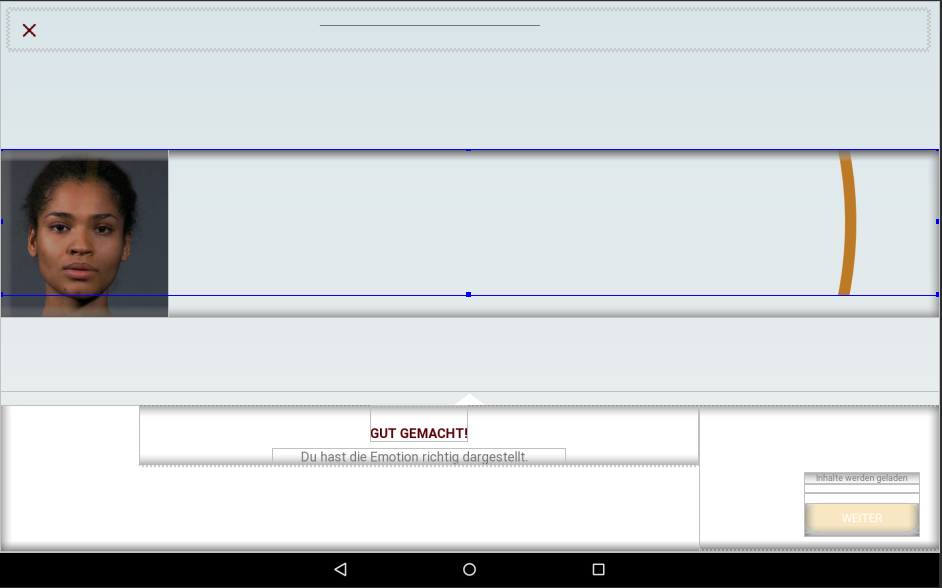
\includegraphics[width=200pt]{res/1.PNG}
\caption{Bildbeschreibung}
\end{figure}

\subsubsection{Wie kann man Intent von dem Fragment?}
\subsubsection{CameraPreviewFragment}
\begin{enumerate}
\item
We could pass the Emotion emotion for a type safety reasons? private int getMaxEmotion(String emotion) switch (emotion)
\item
Are those getters necessary
\subsection{Fragen an Martin}
\item
Das Bild sollte die Frage darstellen
\end{enumerate}
\begin{figure}
\centering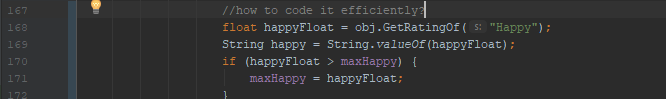
\includegraphics[width=200pt]{res/setMaxHappy.PNG}
\caption{Bildbeschreibung}
\end{figure}

%\end{}
%\vfill
%
\includegraphics[width=2cm]{res/uni_potsdam_logo.pdf}
\subsubsection{Wie kann man Bilder in Latex hinzufügen}
\paragraph{TestBlaubi}
Bailey

\begin{figure}
\centering
\includegraphics[width=200pt]{res/blaubi.PNG}
\caption{Bildbeschreibung}
\end{figure}


\subsubsection{Abstand bei dem Titel vergößsern, vielleicht ein newline Zeichen? Aber wo?}
\paragraph{}Man kann einfach \\ an verschiedenen Stellen hinzufügen

\subsection{TODO:}
\begin{enumerate}
    \item JAVADOC wiederholen
    \item Tobias den Link freigeben
    \item TODOs in Android Studio
\end{enumerate}